\chapter{Limits }
\label{limits}

Physics advances largely by replacing complicated systems with
idealized limits: the point particle, the rigid body, the
continuum, the thermodynamic limit, the classical ($\hbar\to0$)
limit. These idealizations are so routine that it is easy to
forget they are genuine limiting procedures, valid only under
conditions that are rarely stated. When a system depends on a
single small (or large) parameter, sending that parameter to its
limiting value is usually harmless. Most interesting problems,
however, carry \emph{two or more} such parameters, and it is a
basic fact of analysis that iterated limits need not commute:
$\lim_{\varepsilon\to0}\lim_{\delta\to0} f$ can differ from
$\lim_{\delta\to0}\lim_{\varepsilon\to0} f$, or the joint limit
may fail to exist at all. We study this phenomenon through three
worked examples: a beam resting on three rigid pillars, whose
reaction forces depend on whether the beam or the pillars are
idealized as rigid first; Frenkel's classical point electron,
whose self-energy, electromagnetic mass, and radiation-reaction
dynamics depend on the order in which the electron's radius is
sent to zero and its bare mass is renormalized; and the
thermodynamic limit in statistical mechanics, where spontaneous
magnetization exists only if the system-size limit is taken
\emph{before} the symmetry-breaking field is switched off, never
the other way around. We contrast these with limits that are
safe -- the same point-particle and rigid-body idealizations,
used elsewhere, cause no trouble at all -- and extract a general
diagnostic, rooted in the classical theory of singular
perturbations, for telling in advance which limits are
dangerous.

\section{Introduction}

Physics is, in large part, a science of controlled idealization.
We compute planetary orbits by treating planets as point masses;
we compute the deflection of a loaded shelf by treating steel as
a rigid body; we compute the pressure of a gas by treating
$N\sim10^{23}$ molecules as if $N=\infty$; we compute chemical
bonding by treating nuclei as fixed classical points while
treating electrons quantum mechanically; we recover ray optics
from wave optics by sending the wavelength to zero. Each of
these is a genuine mathematical limit -- of a size, a
compliance, an inverse particle number, a wavelength -- applied
to a more complete underlying theory. The success of these
idealizations is one of the great practical facts of physics:
point-particle celestial mechanics is accurate to many decimal
places; rigid-body statics designs bridges that stand for a
century; the thermodynamic limit predicts the boiling point of
water.

It is worth asking \emph{why} these limits are safe, because the
answer clarifies exactly when they stop being safe. A limit in a
single parameter, $\varepsilon\to0$, is unproblematic whenever
the quantity of interest is a continuous (indeed usually
analytic) function of $\varepsilon$ near $\varepsilon=0$: the
answer at small but finite $\varepsilon$ differs from the
idealized answer only by a small, controllable correction, and
nothing is lost by setting $\varepsilon=0$ outright. Trouble
begins when a problem depends on \emph{two or more} such
parameters that are idealized together. Elementary analysis
already warns us that double limits need not commute, and, more
importantly for physics, that the two possible iterated limits
can correspond to two entirely different physical scenarios --
because the order in which we idealize encodes an assumption
about which physical mechanism is responsible for resolving
whatever the un-idealized, finite-parameter system needed to
resolve. Get the order wrong, and the model quietly answers a
different question than the one being asked.

\section{The mathematics of non-commuting limits}
\label{limits:math}
The phenomenon  already appears in
single-variable calculus applied to two variables. Consider
\begin{equation}
f(x,y) = \frac{x^2}{x^2+y^2}, \qquad (x,y)\neq(0,0).
\end{equation}
For any fixed $y\neq0$,
\begin{equation}
\lim_{x\to0} f(x,y) = 0 \quad\Longrightarrow\quad
    \lim_{y\to0}\Big(\lim_{x\to0}f(x,y)\Big) = 0,
\end{equation}
while for any fixed $x\neq0$,
\begin{equation}
\lim_{y\to0} f(x,y) = 1 \quad\Longrightarrow\quad
    \lim_{x\to0}\Big(\lim_{y\to0}f(x,y)\Big) = 1.
\end{equation}
The two iterated limits disagree, and in fact the joint limit
$\lim_{(x,y)\to(0,0)}f(x,y)$ does not exist at all: approaching
the origin along the ray $y=\lambda x$ gives $f =
1/(1+\lambda^2)$, a different value for every slope $\lambda$.
There is no way to ``just set $x=y=0$''; the answer one gets
depends entirely on the \emph{path} by which the two small
parameters are sent to zero together.

This is not a pathology invented for textbooks. It is the
generic behavior of a two-parameter limit unless one can show,
in addition to the two iterated limits agreeing, that the
convergence is \emph{uniform} -- that $f(x,y)$ is close to its
limiting value for \emph{all} small $(x,y)$ simultaneously, not
just along special directions. Physical idealizations are
exactly this kind of two-parameter limit whenever a problem
carries two small (or large) quantities -- a size and a
coupling, a compliance and a stiffness, an inverse system size
and a symmetry-breaking field -- that are both being sent to an
extreme value in the course of ``simplifying'' the problem.

The same structure reappears, in disguise, in the classical
theory of \emph{singular perturbations}. Consider a
boundary-value problem such as
\begin{equation}
\varepsilon\, y''(x) + y'(x) = g(x), \qquad y(0)=y_0,\ \ y(1)=y_1,
\end{equation}
with $\varepsilon>0$ small. At $\varepsilon=0$ the equation
degenerates from second order to first order, and a first-order
equation cannot in general satisfy \emph{two} boundary
conditions. The naive limit ``set $\varepsilon=0$'' therefore
does not smoothly approach the true small-$\varepsilon$
solution: instead, the true solution develops a thin
\emph{boundary layer}, near one endpoint, across which $y$
changes rapidly to absorb the boundary condition that the
reduced ($\varepsilon=0$) equation cannot satisfy. Away from the
layer the reduced equation is an excellent approximation; inside
it, it is not. The parameter $\varepsilon$ multiplies the
\emph{highest derivative} in the equation, and it is precisely
this feature -- a small parameter multiplying the term that
carries the extra structure needed to fix an otherwise
under-determined problem -- that signals a dangerous limit. All
three case studies below exhibit this same signature, dressed in
different physical clothing.

\section{The length of the curve}
\label{limits:curve-length}
Important example: two smooth curve may coincide as sets of points, but have
different lengths. Let $ y_n= \sin(n x)/n $ on the  interval $ 0\le x \le 2 \pi $. 
Calculation of length of sinusoidal curve is a simple exercise in elliptic integrals:
\begin{equation}
   \label {sin-length}
   \begin{split}
       l_n=\int_0^{2 \pi}\sqrt{1+\cos^2(nx)}dx\\
       =\int_0^{2 n \pi}\sqrt{1+\cos^2(z)}dz/n\\
       =\int_0^{2 \pi}\sqrt{1+\cos^2(z)}dz\quad \text{does not depend on n}  \\
       =4 \sqrt{2} \int_0^{\pi/2}\sqrt{1-\frac{1}{2} \sin^2(z)}dz\\
       =4 \sqrt{2} E(\frac{1}{\sqrt{2}}) \approx 1.351
   \end{split}
\end{equation}  
and ratio of its length to that of segment is $ \approx 1.22 $ independent of $ n $.
On the other hand maximal distance between the curve and straight segment $ d_n=1/n $ 
vanishes for $ n\rightarrow \infty $.

\section{ The beam on three pillars}
\label{limits:beam}
Contrary to common belief not every properly set problem in
classical mechanics has unique solution. Let's take for example
a (rigid) beam on three (rigid) pillars (see fig.\ref{beam3}).
\begin{figure}[h]
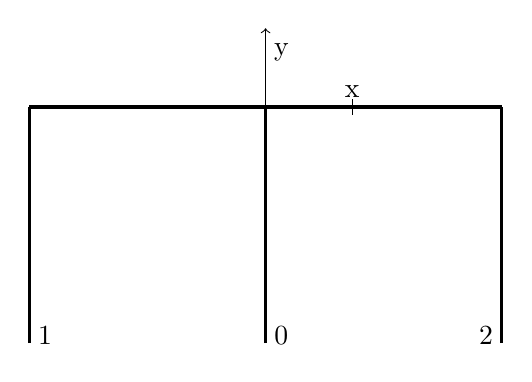
\begin{tikzpicture}
%\draw[thin,dotted] (-3,-3) grid (3,1);
\draw[->] (0,0) -- (0,1);
\node at (0.2,0.7)  {y};
\draw[very thick] (-3,0) -- (3,0);
\draw[very thick] (-3,-3) -- (-3,0);
\draw[very thick] (3,-3) -- (3,0);
\draw[very thick] (0,-3) -- (0,0);
\draw (1.1,-0.1) -- (1.1,0.1);
\node at (1.1,0.2) {x};
\node at (-2.8,-2.9) {1};
\node at (0.2,-2.9) {0};
\node at (2.8,-2.9) {2};
\end{tikzpicture}
\caption{Beam on 3 pillars}
\label {beam3}
\end{figure}
Let the weight of the beam be $W$ and length $2 L$.
Balance of forces gives:
\begin{equation}
        F_0+F_1+F_2=W \label {bf}
\end{equation}
Balance of torques gives:
\begin{equation}
        F_1 L=F_2 L \label {bt}
\end{equation}
   So we have only two equations for three
unknown forces. From the symmetry we can get that $F_1=F_2$. 
(We know that this already from balance of torques.)
{\em First solution}:
All pillars and beam are absolutely rigid. Then
if we pull out the middle pillar nothing will change.
So $F_0=0$ and $F_1=F_2=W/2$.
{\em Second solution}
All pillars and beam are absolutely rigid. Then
we can cat beam at the center and will have two
beams laying on two pillars each.
So $F_0=W/2$ and $F_1=F_2=W/4$.
{\em Third solution}
Beam is absolutely rigid, pillars are very hard springs.
Since beam is horizontal, small change in length is 
equal to all pillars so $F_0=F_1=F_2=w/3$
{\em Fourth solution}
Pillars are rigid, beam is elastic. This case needs
some calculations, well known in elasticity theory
(see e.g \cite {Landau-Lifshitz-7}).
The results is $F_0=5 W/8$ and $F_1=F_2=3 W/16$.
It is clear that all these solutions (and more can be
produced) are limiting cases of standard elasticity 
problem when elasticity coefficients go to infinity.
So generally we can't simply neglect elastic deformations,
we should be more careful.

\section{ The rigid-body limit}
\label{limits:rb}
A perfectly rigid body is often defined by the condition that distances between
material points remain fixed:
$|\mathbf{x}_A-\mathbf{x}_B|=\mathrm{const}$.
Real solids satisfy this only approximately.
For an elastic body, deformation is controlled by elastic moduli, density,
geometry, loading rate, and boundary conditions. A naive rigid-body limit might
be written $E\rightarrow\infty$.
But another relevant quantity is the elastic wave speed 
\[c_s\sim\sqrt{\frac{E}{\rho}}.\]
Thus $E\rightarrow\infty$ typically implies $c_s\rightarrow\infty$
if density is held fixed.
Consequently, the rigid-body limit simultaneously contains an assumption of
infinitely rapid propagation of stress.
If the characteristic time of observation is $T$ and the body size is $L$, 
then the important parameter is
\[\epsilon=\frac{L/c_s}{T}.\]
The rigid approximation corresponds to $\epsilon\ll 1$.
But this can be achieved in different ways:
\[c_s\rightarrow\infty\quad\text{at fixed }L,T,\]
or
\[T\rightarrow\infty\quad\text{at fixed }c_s,L,\]
or through correlated scalings.
These limits need not be equivalent in dynamical problems.

Relativity introduces an additional obstruction. No physical disturbance can 
propagate faster than $c$.
A strictly rigid relativistic body in the Newtonian sense would require
instantaneous transmission of constraints and is therefore incompatible with
relativistic causality.
The successful rigid-body approximation is consequently an asymptotic regime:
\[\frac{L}{c_s T}\ll 1,\]
with $c_s<c$.
Thus the nonrelativistic rigid body is not literally a material object of
infinite stiffness. It is an effective description valid when elastic
transients are irrelevant to the phenomena being studied.
The distinction between an exact ideal object and a controlled asymptotic
approximation is crucial.

\section{Frenkel's point electron}
\label{limits:frenkel}
\subsection{Self-energy and the point limit}

Model the electron classically as a charge $e$ spread over a
sphere of radius $r_0$. The electrostatic self-energy is
(Gaussian units)
\begin{equation}
U(r_0) = \kappa\,\frac{e^2}{r_0}, \qquad \kappa = O(1)
\end{equation}
( $\kappa=\tfrac12$ for a thin shell,$\kappa=\tfrac35$ for a uniform solid sphere),
which diverges as $r_0\to0$. If this self-energy is attributed
entirely to the field's inertia, one obtains an
``electromagnetic mass'' -- but the value one gets depends on
\emph{how} it is computed. From the field momentum of a slowly
moving charged sphere, $p_{\rm em}=\tfrac{4}{3}(U/c^2)v$, so
that $p=m_{\rm em}v$ gives 
$m_{\rm em}^{(p)}=\tfrac{4}{3}U/c^2$;
from the energy directly, $m_{\rm em}^{(E)}=U/c^2$. The mismatch
by a factor of $4/3$ is the classic \emph{$4/3$ problem}: a
purely electromagnetic self-energy is not, on its own,
consistent with relativistic energy-momentum bookkeeping. It is
resolved (Poincar\'e) by recognizing that a charge distribution
held together against its own Coulomb repulsion needs a
non-electromagnetic cohesive stress, and that stress's own
energy and momentum supply exactly the missing $-\tfrac13$,
restoring $m_{\rm total}=E_{\rm total}/c^2$. The lesson for the
present paper is direct: ``send $r_0\to0$'' is not, by itself, a
well-defined instruction until one has also decided how the
(divergent) self-energy is to be renormalized against a second,
independently divergent quantity -- here, the binding stress.

\subsection{Mass renormalization: two divergences, one limit}

The point-particle idealization becomes fully explicit, and fully
double-parametered, once we ask for the electron's \emph{total} inertial mass.
Write the observed mass as
\begin{equation}
m = m_0(r_0) + \frac{U(r_0)}{c^2} = m_0(r_0) + \kappa\,\frac{e^2}{r_0 c^2},
\end{equation}
where $m_0(r_0)$ is a ``bare'' mechanical mass attributed to
whatever holds the charge together. The point limit $r_0\to0$ is
only physically sensible if it is taken \emph{together} with
$m_0(r_0)\to-\infty$ at a matched rate, $m_0(r_0) = m - \kappa
e^2/(r_0c^2) + O(r_0)$, so that the finite, measured mass $m$
survives. This is nothing other than the electromagnetic
prototype of mass renormalization later central to quantum field
theory: a single, uncorrelated limit $r_0\to0$ is meaningless
(it sends $U/c^2\to\infty$), while the \emph{correlated} double
limit, in which $r_0\to0$ and $m_0\to-\infty$ are locked
together so that their sum stays fixed, is perfectly well
defined. Once again, the naive single-parameter idealization
(``the electron is a point'') silently presupposes a highly
specific joint limit in a second, hidden parameter.

\subsection{Radiation reaction}

Expanding the retarded self-force on a small but finite charged sphere in
powers of $r_0$ and taking $r_0\to0$ together with the mass renormalization
above yields, to leading order, the Abraham--Lorentz equation of motion
\begin{equation}
m\,\dot{\vec v} = \vec F_{\rm ext} + \frac{2e^2}{3c^3}\,\ddot{\vec v},
\label{eq:AL}
\end{equation}
where $\dot{\vec v}$ is the acceleration and $\ddot{\vec v}$ its
time derivative (the ``jerk''). Because it involves $\ddot{\vec
v}$, Eq.~\eqref{eq:AL} is effectively a \emph{third}-order
equation of motion for the position, in contrast to Newton's
second-order $m\dot{\vec v}=\vec F$. This raises the order of the
equation exactly as $\varepsilon\to0$ lowered the order of the
boundary-layer equation -- here the point limit
\emph{increases} the number of initial conditions needed, and
the extra solutions it admits are unphysical: Eq.~\eqref{eq:AL}
has runaway solutions that self-accelerate exponentially even
with $\vec F_{\rm ext}=0$, and demanding that these be excluded
forces the physical solutions into \emph{pre-acceleration} --
the particle begins to respond to a force an interval
$\tau=2e^2/(3mc^3)$ (of order $10^{-24}\,$s for the physical
electron) \emph{before} the force is applied, a mild but genuine
violation of naive causality on that timescale.

Both pathologies -- runaway solutions and pre-acceleration --
are artifacts of having taken $r_0\to0$ specifically \emph{in
the radiation-reaction term}, before the internal structure of
the charge has had a chance to regularize the self-force at
short times. Keeping $r_0$ finite removes both problems (at the
cost of reintroducing internal structural dynamics that must
themselves be modeled), just as keeping stiffness $EI$ or $k$ finite
removed the indeterminacy of the beam in section \ref{limits:beam}.
This is precisely the
sense in which the point-particle limit is \emph{singular} for
the specific question ``what is the self-consistent equation of
motion including radiation reaction?''

It is worth emphasizing, by contrast, that the very same point
limit is completely \emph{safe} for other questions about the
same object: Rutherford scattering, planetary-orbit-style
Coulomb dynamics, and multipole expansions of the field far from
the charge all depend on $r_0$ only through smooth, subdominant
corrections of relative size $(r_0/L)^n$, where $L$ is the
relevant external length scale, and these corrections vanish
continuously as $r_0\to0$ with no hidden second parameter
involved. The point-electron idealization is thus simultaneously
excellent (for scattering and orbits) and treacherous (for
self-energy and radiation reaction) -- the difference is
entirely about \emph{which question is being asked}, not about
the idealization itself. Frenkel's own 1926 model of a
relativistic, spinning point electron sits squarely in this
tradition: it sidesteps the internal-structure question by fiat
(endowing the point particle with an intrinsic spin and magnetic
moment rather than deriving them from a charge distribution),
buying calculability at the price of leaving the self-energy and
radiation-reaction issues exactly where the discussion above
leaves them.

\section{The thermodynamic limit and spontaneous magnetization}
\label{limits:td}
For a magnetic system of $N$ spins in an external field $h$ at
temperature $T$, the partition function $Z_N(T,h)$ is a finite
sum of exponentials of the spin configuration energies, hence an
entire (analytic) function of $h$ and $T$ for every finite $N$.
In particular, for $h=0$ the up--down symmetry of the
Hamiltonian forces the average magnetization per spin to vanish
\emph{exactly} for every finite $N$:
\begin{equation}
m(T,h=0,N) = 0 \qquad \text{for all finite } N.
\end{equation}
Yet real ferromagnets below their Curie temperature $T_c$
exhibit a nonzero \emph{spontaneous} magnetization at zero
field. The resolution is again a matter of the order of two
limits. Define
\begin{equation}
m_s(T) \equiv \lim_{h\to0^+}\ \lim_{N\to\infty}\ m(T,h,N).
\end{equation}
For $T<T_c$ this limit is nonzero: sending $N\to\infty$
\emph{first}, at fixed small $h>0$, allows the free-energy
landscape to develop two deep, well-separated minima (``up'' and
``down''), and the infinite system, prepared with an
infinitesimal field, is trapped in one of them even after the
field is switched off. But the \emph{opposite} order,
\begin{equation}
\lim_{N\to\infty}\ \lim_{h\to0}\ m(T,h,N) = \lim_{N\to\infty} 0 = 0,
\end{equation}
gives identically zero at every temperature, because the inner
limit is zero for every finite $N$ by the symmetry argument
above. Spontaneous symmetry breaking is, in this precise sense,
only ever visible in one of the two iterated limits: the
thermodynamic limit must be taken \emph{before} the
symmetry-breaking field is removed, never after. A closely
related statement is the Lee--Yang picture of phase transitions:
the zeros of $Z_N$ in the complex-field plane are, for finite
$N$, always off the physical (real) axis, so that $Z_N$ and all
its finite-$N$ thermodynamic functions are perfectly smooth; a
genuine non-analyticity -- a true phase transition -- can only
appear where those zeros pinch the real axis as $N\to\infty$.
Once again, a physically essential phenomenon (ferromagnetism,
phase transitions generally) is invisible unless a particular
one of two possible iterated limits is used, and the finite-$N$,
finite-$h$ system does not, by itself, tell you which order is
the physically relevant one; that has to be supplied from
outside, by the physical fact that real magnets are prepared in
one broken-symmetry state at a time, not in a symmetric
superposition of both.

\section{Continuum limit versus point-particle limit}
At first sight, the point-particle limit and the continuum limit appear opposite.
The point-particle limit removes internal spatial structure:
$R/L\rightarrow 0$. The continuum limit removes microscopic granularity:
$\ell_{\rm micro}/L\rightarrow 0$.
But both are examples of scale separation.

Suppose a system contains
$\ell_{\rm micro}\ll R \ll L$.
Then one may first construct a continuum description of an extended object,
$\ell_{\rm micro}/R\rightarrow 0$,
and subsequently approximate that object as pointlike,
$R/L\rightarrow 0$.

These operations may be interchangeable only if there exists an overlap region satisfying
$\ell_{\rm micro}\ll R \ll L$.
If this hierarchy collapses, the two approximations can interfere.
For example, if $R\rightarrow 0$ is taken so rapidly that $R\sim\ell_{\rm micro}$,
then the continuum description loses validity before the point-particle approximation is reached.
Thus continuum limit followed by point limit need not equal the reverse procedure.
The existence of a useful intermediate scale is often what makes successive idealizations legitimate.

\section{Thermodynamic and long-time limits}
The thermodynamic limit is another central example.
For a finite system,$N<\infty$,
the partition function is generally analytic under ordinary conditions. Sharp phase 
transitions emerge only in an infinite-system limit.
Schematically,$\lim_{N\rightarrow\infty}$
may produce nonanalytic behavior that is absent for every finite $N$.
Now introduce the long-time limit, $t\rightarrow\infty$.
The two limits $N\rightarrow\infty$ and $t\rightarrow\infty$
can be highly nontrivial.

For finite $N$, a Hamiltonian system may exhibit recurrences on sufficiently
long times. If the thermodynamic limit is taken first, recurrence times may
diverge and irreversible behavior can emerge at the level of effective
descriptions.
Thus one encounters the conceptual contrast
$\lim_{t\to\infty}\lim_{N\to\infty}$ versus $\lim_{N\to\infty}\lim_{t\to\infty}$.
The relation between these procedures is central to the foundations of statistical mechanics and the emergence of irreversibility.
The phrase \emph{take the thermodynamic limit} therefore conceals assumptions 
concerning observation time, coarse graining, boundary conditions, and the 
class of states being considered.

\section{Zero temperature and infinite volume}
Quantum and statistical systems often involve the pair
$T\rightarrow 0,\qquad V\rightarrow\infty$.
At finite volume, energy levels are generally discrete. In the infinite-volume limit, 
spectra may become continuous or dense.
The ground-state structure can therefore depend subtly on the order of limits.
Similarly, spontaneous symmetry breaking is sharply formulated only after an
infinite-volume or thermodynamic limit is invoked. For finite systems,
symmetry-related states can tunnel into one another, and exact eigenstates may
retain the symmetry of the Hamiltonian.

The usual conceptual sequence is often
$V\rightarrow\infty$,
followed by the removal of an infinitesimal symmetry-breaking source,
$h\rightarrow 0$.
The order
\[\lim_{h\to0}\lim_{V\to\infty}\]
can differ from
\[\lim_{V\to\infty}\lim_{h\to0}.\]

This is not a mathematical curiosity. It expresses the physical distinction between:
 first selecting a macroscopic phase and then removing the external bias;
 first removing the bias in a finite symmetric system and only then increasing the size.
Thus spontaneous symmetry breaking itself provides a paradigmatic example of noncommuting limits.

\section{The classical limit: $\hbar\to 0$ is not a universal procedure}
The statement that classical mechanics is obtained by taking
$\hbar\rightarrow 0$ is useful but incomplete.
The physically relevant semiclassical parameter is typically an action ratio,
\[\epsilon_{\rm sc}=\frac{\hbar}{S_{\rm cl}}.\]
Thus the classical regime may be reached through large actions rather than a literal variation of Planck's constant.
Moreover, another parameter may be time.
Semiclassical approximations are frequently valid only over restricted time scales. In chaotic systems, small quantum corrections may grow under classical instability.
Thus $\hbar\rightarrow 0$ and $t\rightarrow\infty$ may not commute.
For fixed finite $t$, $\lim_{\hbar\to0}$ 
may reproduce classical dynamics.
But if $t$ increases simultaneously with decreasing $\hbar$, 
interference and quantum corrections can become important.
The appropriate question is therefore not simply
"$\hbar\rightarrow 0$?" but rather "$\frac{\hbar}{S}\rightarrow 0 \quad\text{with what scaling of }t$?"

This illustrates a general principle:
 A limiting theory may be valid at every fixed value of a second variable and nevertheless fail to be uniformly valid as that second variable also approaches an extreme regime.

\section{ The Newtonian limit and weak-field limit}
Relativity provides another multiparameter example.
A nonrelativistic weak-field regime may involve
$\frac{v}{c}\ll 1,\qquad \frac{GM}{rc^2}\ll 1$.
It is tempting to regard these as independent.
However, different physical systems can approach the joint Newtonian regime along very different paths.
A system may have $v/c\ll 1$ but still experience strong gravitational fields, or conversely 
have weak gravity while containing ultrarelativistic particles.
Thus $c\rightarrow\infty$ and $G\rightarrow 0$
are not conceptually identical limiting procedures.
One may define different contractions or scaling limits depending on which combinations of parameters are held fixed.

Similarly, the limits $c\rightarrow\infty,\qquad\hbar\rightarrow 0$
raise a further question:
\[\text{Does classical mechanics arise before or after the nonrelativistic limit?}\]
In ordinary regimes the resulting descriptions overlap and agree. But the mathematical limiting structures need not be identical, especially when spin, antiparticles, constraints, or quantum fields are involved.
\section{Why some limits are safe}
\label{limits:safe}
The three case studies above should not be read as an indictment
of point-particle or rigid-body idealizations in general -- both
are used successfully, constantly, throughout physics. What
distinguishes a safe use from a dangerous one is not the
idealization itself but the \emph{role} the discarded parameter
was playing in the finite theory.

\begin{principle}
A limiting idealization is safe (the order of limits does not
    matter, and a single limit suffices) when the discarded
    parameter enters the quantity of interest only as a smooth,
    subdominant correction that vanishes continuously as the
    parameter is removed.
\end{principle}

This is exactly the situation in planetary mechanics (finite
planetary radius enters orbital dynamics only through small,
regular tidal and multipole corrections), in Rutherford-style
scattering (finite nuclear size enters the cross-section as a
regular form-factor correction, negligible when the probe
wavelength is much larger than the nucleus), and in ordinary,
\emph{statically determinate} rigid-body mechanics, where the
number of unknown constraint forces already matches the number
of equilibrium equations before any compliance is introduced, so
elastic corrections enter as small, regular shifts rather than
as the sole source of a missing equation. The thermodynamic
limit is likewise safe for the overwhelming majority of bulk
thermodynamic quantities -- the equation of state, the specific
heat away from a critical point, the equilibrium constant of a
chemical reaction -- because these depend smoothly on $1/N$ and
converge to the same value regardless of how any auxiliary field
is handled.

\begin{principle}
A limiting idealization is dangerous when the discarded
    parameter is doing one of three jobs in the finite theory:
    (i) resolving a redundancy or degeneracy (a statically
    indeterminate structure, a degenerate ground-state
    manifold); (ii) regularizing a formally divergent,
    self-referential quantity (a self-energy, a self-force); or
    (iii) selecting among multiple locally stable branches or
    vacua (spontaneous symmetry breaking, runaway versus
    physical solutions of an equation of motion).
\end{principle}

All three case studies above instantiate exactly one of these
three roles: the beam's redundancy (i), the point electron's
self-energy and self-force (ii), and the ferromagnet's broken
symmetry (iii).

\section{A diagnostic for dangerous limits}
\label{limits:danger}
The discussion above suggests a short, practical checklist for
deciding, in advance, whether a proposed idealization is likely
to be safe.

\begin{enumerate}
\item \textbf{Count the constraints.} If the idealized (e.g.\
    rigid, point-like) description leaves more unknowns than
        equations -- a redundancy -- some discarded compliance
        is doing essential work, and the idealization must be
        taken only after that compliance has fixed the
        redundancy.
\item \textbf{Look for self-reference.} If the quantity of
    interest involves a source acting on its own field, or any
        other quantity that diverges as the idealization is
        approached, expect a second, compensating divergence (a
        bare mass, a counterterm, a binding stress) that must be
        tracked through the same limit.
\item \textbf{Look for a symmetry that would force a trivial
    answer.} If an exact symmetry of the un-idealized, finite
        system would make the naive order of limits give zero
        (or some other symmetric, ``un-broken'' value) by fiat,
        check whether the physically relevant answer instead
        requires the symmetry-breaking parameter to be removed
        only \emph{after} the idealizing limit.
\item \textbf{Check whether the discarded parameter multiplies
    the highest derivative} in the governing equation (as $EI$
        does in the beam equation, or as the internal structure
        of a charge does in the retarded self-force). If so, the
        limit is a singular perturbation, and a boundary layer,
        runaway mode, or other qualitative change in the
        solution set should be expected.
\item \textbf{When in doubt, compute along more than one path.}
    If a two-(or more)-parameter idealization gives different
        answers along different paths to the same nominal limit
        (as in the toy example of Section~2), the safe procedure
        is to keep the physically relevant ratio of the two
        parameters fixed at its true, finite value, rather than
        sending either parameter to infinity ``first.''
\end{enumerate}

None of this is a reason to distrust idealization as a method;
it is, if anything, a reason to trust it more, because it turns
an occasional embarrassing paradox (a beam problem with no
unique answer, an electron with infinite self-energy, a
symmetric theory that somehow predicts a magnet) into a routine
calculation once the second, hidden parameter is identified and
tracked through the limit alongside the first.

\section{Conclusion}
\label{limits:conclusion}
Idealized limits are indispensable, and in the great majority of
their uses they are also perfectly safe: the point particle, the
rigid body, the continuum, and the thermodynamic limit each work
because the physics they discard enters only as a small, smooth
correction. But whenever an idealizing parameter is secretly
doing double duty -- resolving a redundancy, regularizing a
self-interaction, or selecting a symmetry-broken branch -- the
limit becomes a genuine two-(or more-)parameter limit in the
technical sense of Section~2, and the order in which the
idealizations are imposed is no longer a matter of convenience
but a physical assumption in its own right, one that must be
justified by the actual mechanism operating in the un-idealized
system. The beam on three pillars, the point electron, and the
thermodynamic limit of a ferromagnet each illustrate a different
flavor of this same structure -- static redundancy,
field-theoretic self-reference, and spontaneous symmetry
breaking, respectively -- and, not coincidentally, each
historically forced the development of new formal machinery (the
force method and compatibility conditions in structural
mechanics; mass renormalization in classical and later quantum
field theory; the Lee--Yang theory of phase transitions in
statistical mechanics) precisely in order to tame it.
Recognizing the common mathematical skeleton beneath these
episodes -- non-commuting iterated limits, in the elementary
sense of Section~2 -- is a useful piece of general-purpose
intuition for noticing, before the paradox appears, when an
idealization needs a second parameter kept on a leash.

